% Created by tikzDevice version 0.10.1 on 2016-08-15 14:44:54
% !TEX encoding = UTF-8 Unicode
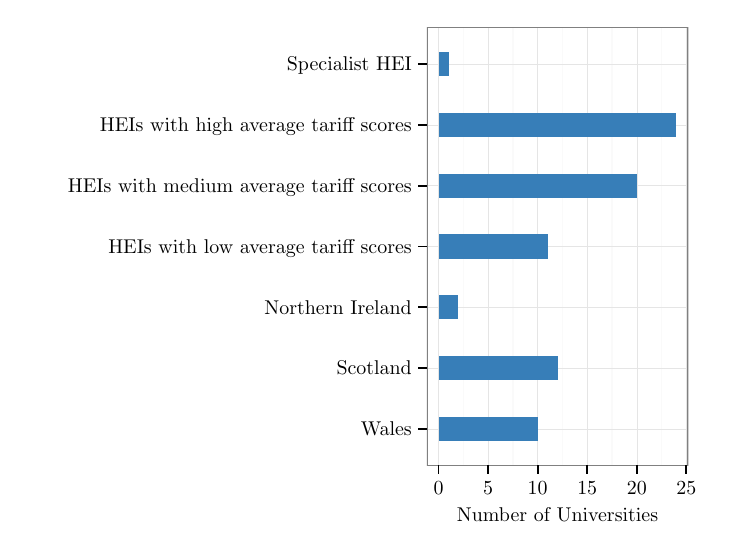
\begin{tikzpicture}[x=1pt,y=1pt]
\definecolor{fillColor}{RGB}{255,255,255}
\path[use as bounding box,fill=fillColor,fill opacity=0.00] (0,0) rectangle (252.94,180.67);
\begin{scope}
\path[clip] (  0.00,  0.00) rectangle (252.94,180.67);
\definecolor{drawColor}{RGB}{255,255,255}
\definecolor{fillColor}{RGB}{255,255,255}

\path[draw=drawColor,line width= 0.6pt,line join=round,line cap=round,fill=fillColor] (  0.00,  0.00) rectangle (252.94,180.68);
\end{scope}
\begin{scope}
\path[clip] (144.21, 22.52) rectangle (238.72,180.67);
\definecolor{fillColor}{RGB}{255,255,255}

\path[fill=fillColor] (144.21, 22.52) rectangle (238.72,180.67);
\definecolor{drawColor}{gray}{0.98}

\path[draw=drawColor,line width= 0.6pt,line join=round] (157.45, 22.52) --
	(157.45,180.67);

\path[draw=drawColor,line width= 0.6pt,line join=round] (175.35, 22.52) --
	(175.35,180.67);

\path[draw=drawColor,line width= 0.6pt,line join=round] (193.25, 22.52) --
	(193.25,180.67);

\path[draw=drawColor,line width= 0.6pt,line join=round] (211.15, 22.52) --
	(211.15,180.67);

\path[draw=drawColor,line width= 0.6pt,line join=round] (229.05, 22.52) --
	(229.05,180.67);
\definecolor{drawColor}{gray}{0.90}

\path[draw=drawColor,line width= 0.2pt,line join=round] (144.21, 35.70) --
	(238.72, 35.70);

\path[draw=drawColor,line width= 0.2pt,line join=round] (144.21, 57.66) --
	(238.72, 57.66);

\path[draw=drawColor,line width= 0.2pt,line join=round] (144.21, 79.63) --
	(238.72, 79.63);

\path[draw=drawColor,line width= 0.2pt,line join=round] (144.21,101.60) --
	(238.72,101.60);

\path[draw=drawColor,line width= 0.2pt,line join=round] (144.21,123.56) --
	(238.72,123.56);

\path[draw=drawColor,line width= 0.2pt,line join=round] (144.21,145.53) --
	(238.72,145.53);

\path[draw=drawColor,line width= 0.2pt,line join=round] (144.21,167.50) --
	(238.72,167.50);

\path[draw=drawColor,line width= 0.2pt,line join=round] (148.50, 22.52) --
	(148.50,180.67);

\path[draw=drawColor,line width= 0.2pt,line join=round] (166.40, 22.52) --
	(166.40,180.67);

\path[draw=drawColor,line width= 0.2pt,line join=round] (184.30, 22.52) --
	(184.30,180.67);

\path[draw=drawColor,line width= 0.2pt,line join=round] (202.20, 22.52) --
	(202.20,180.67);

\path[draw=drawColor,line width= 0.2pt,line join=round] (220.10, 22.52) --
	(220.10,180.67);

\path[draw=drawColor,line width= 0.2pt,line join=round] (238.00, 22.52) --
	(238.00,180.67);
\definecolor{fillColor}{RGB}{55,126,184}

\path[fill=fillColor] (148.50, 31.30) rectangle (184.30, 40.09);

\path[fill=fillColor] (148.50, 53.27) rectangle (191.46, 62.06);

\path[fill=fillColor] (148.50, 75.24) rectangle (155.66, 84.02);

\path[fill=fillColor] (148.50, 97.20) rectangle (187.88,105.99);

\path[fill=fillColor] (148.50,119.17) rectangle (220.10,127.96);

\path[fill=fillColor] (148.50,141.14) rectangle (234.42,149.92);

\path[fill=fillColor] (148.50,163.10) rectangle (152.08,171.89);
\definecolor{drawColor}{gray}{0.50}

\path[draw=drawColor,line width= 0.6pt,line join=round,line cap=round] (144.21, 22.52) rectangle (238.72,180.67);
\end{scope}
\begin{scope}
\path[clip] (  0.00,  0.00) rectangle (252.94,180.67);
\definecolor{drawColor}{RGB}{0,0,0}

\node[text=drawColor,anchor=base east,inner sep=0pt, outer sep=0pt, scale=  0.72] at (138.81, 33.22) {Wales};

\node[text=drawColor,anchor=base east,inner sep=0pt, outer sep=0pt, scale=  0.72] at (138.81, 55.18) {Scotland};

\node[text=drawColor,anchor=base east,inner sep=0pt, outer sep=0pt, scale=  0.72] at (138.81, 77.15) {Northern Ireland};

\node[text=drawColor,anchor=base east,inner sep=0pt, outer sep=0pt, scale=  0.72] at (138.81, 99.12) {HEIs with low average tariff scores};

\node[text=drawColor,anchor=base east,inner sep=0pt, outer sep=0pt, scale=  0.72] at (138.81,121.08) {~HEIs with medium average tariff scores};

\node[text=drawColor,anchor=base east,inner sep=0pt, outer sep=0pt, scale=  0.72] at (138.81,143.05) {HEIs with high average tariff scores};

\node[text=drawColor,anchor=base east,inner sep=0pt, outer sep=0pt, scale=  0.72] at (138.81,165.02) {Specialist HEI};
\end{scope}
\begin{scope}
\path[clip] (  0.00,  0.00) rectangle (252.94,180.67);
\definecolor{drawColor}{RGB}{0,0,0}

\path[draw=drawColor,line width= 0.6pt,line join=round] (141.21, 35.70) --
	(144.21, 35.70);

\path[draw=drawColor,line width= 0.6pt,line join=round] (141.21, 57.66) --
	(144.21, 57.66);

\path[draw=drawColor,line width= 0.6pt,line join=round] (141.21, 79.63) --
	(144.21, 79.63);

\path[draw=drawColor,line width= 0.6pt,line join=round] (141.21,101.60) --
	(144.21,101.60);

\path[draw=drawColor,line width= 0.6pt,line join=round] (141.21,123.56) --
	(144.21,123.56);

\path[draw=drawColor,line width= 0.6pt,line join=round] (141.21,145.53) --
	(144.21,145.53);

\path[draw=drawColor,line width= 0.6pt,line join=round] (141.21,167.50) --
	(144.21,167.50);
\end{scope}
\begin{scope}
\path[clip] (  0.00,  0.00) rectangle (252.94,180.67);
\definecolor{drawColor}{RGB}{0,0,0}

\path[draw=drawColor,line width= 0.6pt,line join=round] (148.50, 19.52) --
	(148.50, 22.52);

\path[draw=drawColor,line width= 0.6pt,line join=round] (166.40, 19.52) --
	(166.40, 22.52);

\path[draw=drawColor,line width= 0.6pt,line join=round] (184.30, 19.52) --
	(184.30, 22.52);

\path[draw=drawColor,line width= 0.6pt,line join=round] (202.20, 19.52) --
	(202.20, 22.52);

\path[draw=drawColor,line width= 0.6pt,line join=round] (220.10, 19.52) --
	(220.10, 22.52);

\path[draw=drawColor,line width= 0.6pt,line join=round] (238.00, 19.52) --
	(238.00, 22.52);
\end{scope}
\begin{scope}
\path[clip] (  0.00,  0.00) rectangle (252.94,180.67);
\definecolor{drawColor}{RGB}{0,0,0}

\node[text=drawColor,anchor=base,inner sep=0pt, outer sep=0pt, scale=  0.72] at (148.50, 12.16) {0};

\node[text=drawColor,anchor=base,inner sep=0pt, outer sep=0pt, scale=  0.72] at (166.40, 12.16) {5};

\node[text=drawColor,anchor=base,inner sep=0pt, outer sep=0pt, scale=  0.72] at (184.30, 12.16) {10};

\node[text=drawColor,anchor=base,inner sep=0pt, outer sep=0pt, scale=  0.72] at (202.20, 12.16) {15};

\node[text=drawColor,anchor=base,inner sep=0pt, outer sep=0pt, scale=  0.72] at (220.10, 12.16) {20};

\node[text=drawColor,anchor=base,inner sep=0pt, outer sep=0pt, scale=  0.72] at (238.00, 12.16) {25};
\end{scope}
\begin{scope}
\path[clip] (  0.00,  0.00) rectangle (252.94,180.67);
\definecolor{drawColor}{RGB}{0,0,0}

\node[text=drawColor,anchor=base,inner sep=0pt, outer sep=0pt, scale=  0.72] at (191.46,  2.40) {Number of Universities};
\end{scope}
\end{tikzpicture}
